\documentclass[aspectratio=169,11pt]{beamer}

\usetheme{metropolis}
\usecolortheme{dolphin}
\usefonttheme{professionalfonts}

\usepackage[T1]{fontenc}
\usepackage[utf8]{inputenc}
\usepackage{lmodern}
\usepackage{amsmath,amssymb}
\usepackage{booktabs}
\usepackage{graphicx}
\usepackage{tikz}
\usetikzlibrary{arrows.meta,positioning,calc,shapes.geometric,fit}

\graphicspath{{assets/}{/Users/ingridcorobana/Desktop/optimizingInlining/out/figures/}{/Users/ingridcorobana/Desktop/optimizingInlining/out/demo/}}

\definecolor{caiBlue}{RGB}{20,73,118}
\definecolor{caiGreen}{RGB}{42,130,111}
\definecolor{caiRed}{RGB}{180,72,63}
\definecolor{caiGold}{RGB}{184,135,49}
\definecolor{softGray}{RGB}{246,248,250}
\definecolor{textGray}{RGB}{55,65,81}

\setbeamercolor{normal text}{fg=textGray,bg=white}
\setbeamercolor{frametitle}{fg=caiBlue,bg=white}
\setbeamercolor{progress bar}{fg=caiGreen,bg=softGray}
\setbeamercolor{alerted text}{fg=caiRed}
\setbeamertemplate{itemize item}{\color{caiGreen}$\blacktriangleright$}
\setbeamertemplate{itemize subitem}{\color{caiGold}$\circ$}
\setbeamertemplate{navigation symbols}{}

\tikzset{
  box/.style={rounded corners=2pt, draw=caiBlue!55, fill=softGray, thick, align=center,
              minimum height=8mm, inner sep=4pt, font=\small},
  greenbox/.style={box, draw=caiGreen!70, fill=caiGreen!8},
  redbox/.style={box, draw=caiRed!70, fill=caiRed!7},
  goldbox/.style={box, draw=caiGold!75, fill=caiGold!10},
  arrow/.style={-{Latex[length=2.2mm]}, thick, draw=caiBlue!75},
  lightarrow/.style={-{Latex[length=2.2mm]}, thick, draw=caiGreen!75}
}

\newcommand{\cppkw}[1]{\textcolor{caiBlue}{\textbf{#1}}}
\newcommand{\cpptype}[1]{\textcolor{caiGreen!75!black}{\textbf{#1}}}
\newcommand{\cppfn}[1]{\textcolor{caiGold!90!black}{#1}}
\newcommand{\cppnum}[1]{\textcolor{caiRed!85!black}{#1}}
\newcommand{\cppcom}[1]{\textcolor{textGray!65}{\itshape #1}}

\title{Optimizarea deciziei de inlining în compilare\\prin tehnici de Machine Learning}
\subtitle{}
\author{Ingrid-Adriana Corobană}
\institute{Profesor coordonator\\Prof. Dr. Cristian Rusu}
\date{}

\begin{document}

\begin{frame}[plain]
\vspace{0.65cm}
\begin{center}
{\Large\bfseries Optimizarea deciziei de inlining în compilare\\[0.15cm]prin tehnici de Machine Learning}

\vspace{0.35cm}
{\normalsize\itshape Inlining Compiler Optimization\\Through Machine Learning Techniques}

\vspace{0.85cm}
\begin{columns}[T,onlytextwidth]
\begin{column}{0.48\textwidth}
\centering
{\normalsize Absolventă}\\[0.12cm]
{\large Ingrid-Adriana Corobană}
\end{column}
\begin{column}{0.48\textwidth}
\centering
{\normalsize Profesor coordonator}\\[0.12cm]
{\large Prof. Dr. Cristian Rusu}
\end{column}
\end{columns}

\vspace{0.85cm}
{\normalsize Lucrare de licență}
\end{center}
\end{frame}

\begin{frame}{Problema: o decizie locală cu efect global}
\begin{columns}[T,onlytextwidth]
\begin{column}{0.56\textwidth}
\begin{itemize}
  \item La fiecare apel, compilatorul decide: \textbf{inline} sau \textbf{keep}.
  \item Inlining-ul elimină overhead-ul apelului și poate dezvălui optimizări ulterioare.
  \item Poate duplica mult cod, crește binarul și schimba oportunitățile de optimizare.
\end{itemize}
\vspace{0.25cm}
\textbf{Încadrarea proiectului:} fiecare call site devine o decizie a unei euristici, iar euristica este învățată din rezultate măsurate.
\end{column}
\begin{column}{0.40\textwidth}
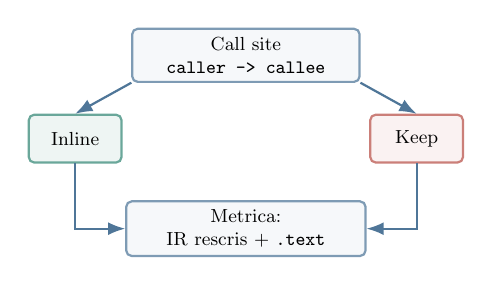
\begin{tikzpicture}[node distance=0.42cm and 0.35cm, scale=0.76, transform shape]
\node[box, minimum width=3.8cm] (call) {Call site\\\texttt{caller -> callee}};
\node[greenbox, below left=0.52cm and 0.15cm of call, minimum width=1.55cm] (yes) {Inline};
\node[redbox, below right=0.52cm and 0.15cm of call, minimum width=1.55cm] (no) {Keep};
\node[box, below=0.62cm of $(yes.south)!0.5!(no.south)$, minimum width=4.0cm] (metric)
{Metrica:\\IR rescris + \texttt{.text}};
\draw[arrow] (call.south west) -- (yes.north);
\draw[arrow] (call.south east) -- (no.north);
\draw[arrow] (yes.south) |- (metric.west);
\draw[arrow] (no.south) |- (metric.east);
\end{tikzpicture}
\end{column}
\end{columns}
\end{frame}

\begin{frame}[shrink=5]{Când ajută și când strică inlining-ul}
\begin{columns}[T,onlytextwidth]
\begin{column}{0.49\textwidth}
\textbf{Bun: propagare de constante}
\vspace{0.15cm}
\begin{center}
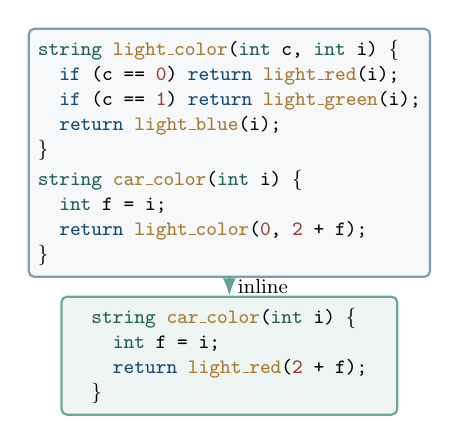
\begin{tikzpicture}[node distance=0.28cm, scale=0.82, transform shape]
\node[box, minimum width=5.2cm, align=left] (before)
{\ttfamily\small
\begin{tabular}{@{}l@{}}
\cpptype{string} \cppfn{light\_color}(\cpptype{int} c, \cpptype{int} i) \{\\
\quad \cppkw{if} (c == \cppnum{0}) \cppkw{return} \cppfn{light\_red}(i);\\
\quad \cppkw{if} (c == \cppnum{1}) \cppkw{return} \cppfn{light\_green}(i);\\
\quad \cppkw{return} \cppfn{light\_blue}(i);\\
\}\\[0.08cm]
\cpptype{string} \cppfn{car\_color}(\cpptype{int} i) \{\\
\quad \cpptype{int} f = i;\\
\quad \cppkw{return} \cppfn{light\_color}(\cppnum{0}, \cppnum{2} + f);\\
\}
\end{tabular}};
\node[greenbox, below=of before, minimum width=5.2cm, align=left] (after)
{\ttfamily\small
\begin{tabular}{@{}l@{}}
\cpptype{string} \cppfn{car\_color}(\cpptype{int} i) \{\\
\quad \cpptype{int} f = i;\\
\quad \cppkw{return} \cppfn{light\_red}(\cppnum{2} + f);\\
\}
\end{tabular}};
\draw[lightarrow] (before) -- node[right, font=\small]{inline} (after);
\end{tikzpicture}
\end{center}
\scriptsize Apelul cu \texttt{c = 0} face ramura relevantă vizibilă pentru optimizări.
\end{column}
\begin{column}{0.49\textwidth}
\textbf{Rău: expansiune recursivă}
\vspace{0.15cm}
\begin{center}
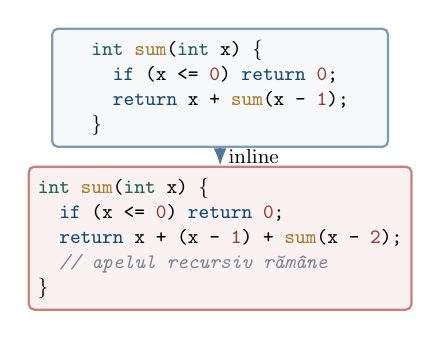
\begin{tikzpicture}[node distance=0.28cm, scale=0.82, transform shape]
\node[box, minimum width=5.2cm, align=left] (before)
{\ttfamily\small
\begin{tabular}{@{}l@{}}
\cpptype{int} \cppfn{sum}(\cpptype{int} x) \{\\
\quad \cppkw{if} (x <= \cppnum{0}) \cppkw{return} \cppnum{0};\\
\quad \cppkw{return} x + \cppfn{sum}(x - \cppnum{1});\\
\}
\end{tabular}};
\node[redbox, below=of before, minimum width=5.2cm, align=left] (after)
{\ttfamily\small
\begin{tabular}{@{}l@{}}
\cpptype{int} \cppfn{sum}(\cpptype{int} x) \{\\
\quad \cppkw{if} (x <= \cppnum{0}) \cppkw{return} \cppnum{0};\\
\quad \cppkw{return} x + (x - \cppnum{1}) + \cppfn{sum}(x - \cppnum{2});\\
\quad \cppcom{// apelul recursiv rămâne}\\
\}
\end{tabular}};
\draw[arrow] (before) -- node[right, font=\small]{inline} (after);
\end{tikzpicture}
\end{center}
\scriptsize Rescrierea expune din nou aceeași structură, deci este nevoie de verificări de recursivitate și creștere.
\end{column}
\end{columns}
\end{frame}

\begin{frame}{Soluție}
\begin{columns}[T,onlytextwidth]
\begin{column}{0.53\textwidth}
\textbf{Ideea principală}
\begin{itemize}
  \item Extrag features pentru fiecare call site din LLVM IR.
  \item Rulez mai multe politici profesor și măsor efectul lor după rescriere.
  \item Aleg cel mai bun profesor pe modul și construiesc un dataset de behavior cloning.
  \item Antrenez modele student care imită deciziile și le evaluez prin rescriere IR.
\end{itemize}
\end{column}
\begin{column}{0.43\textwidth}
\textbf{Contribuția mea}
\begin{itemize}
  \item Pipeline reproductibil end-to-end.
  \item Dataset sintetic plus surse reale.
  \item Politici profesor, selecție BC-Max și modele student.
  \item Evaluare cu artefacte inspectabile.
\end{itemize}
\end{column}
\end{columns}
\vspace{0.18cm}
\centering\textbf{Comanda:} \texttt{python3 scripts/run.py all}
\end{frame}

\begin{frame}{Datele și reprezentarea call site-urilor}
\begin{columns}[T,onlytextwidth]
\begin{column}{0.47\textwidth}
\textbf{Surse}
\begin{itemize}
  \item Snapshot DCMTK: \texttt{config/tests/*.cc}
  \item Module generate determinist pentru cazuri inline-positive și inline-negative
  \item Evaluare separată pe surse reale: 80 module, 9168 eșantioane train/test
\end{itemize}
\end{column}
\begin{column}{0.49\textwidth}
\textbf{Features}
\begin{itemize}
  \item structură caller/callee și cost estimat
  \item număr de utilizatori, înălțime call site, constante în parametri
  \item număr instrucțiuni, număr apeluri și semnal pentru recursivitate
  \item features globale: număr de noduri și muchii în graful de apeluri
\end{itemize}
\end{column}
\end{columns}
\vspace{0.35cm}
\begin{center}
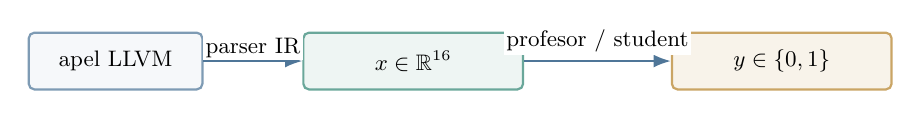
\begin{tikzpicture}[scale=0.9, transform shape]
\node[box, minimum width=2.45cm] (raw) at (0,0) {apel LLVM};
\node[greenbox, minimum width=3.1cm] (vec) at (4.2,0) {$x \in \mathbb{R}^{16}$};
\node[goldbox, minimum width=3.1cm] (action) at (9.4,0) {$y \in \{0,1\}$};
\draw[arrow] (raw.east) -- node[above, midway, font=\small, fill=white, inner sep=1pt]{parser IR} (vec.west);
\draw[arrow] (vec.east) -- node[above=2pt, midway, font=\small, fill=white, inner sep=1pt]{profesor / student} (action.west);
\end{tikzpicture}
\end{center}
\end{frame}

\begin{frame}{Pipeline-ul complet}
\centering
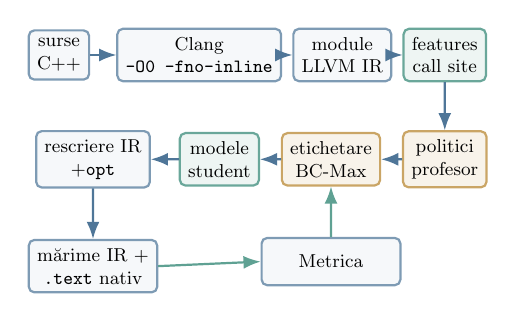
\begin{tikzpicture}[node distance=0.38cm and 0.18cm, scale=0.75, transform shape]
\node[box] (src) {surse\\C++};
\node[box, right=0.45cm of src] (clang) {Clang\\\texttt{-O0 -fno-inline}};
\node[box, right=of clang] (ir) {module\\LLVM IR};
\node[greenbox, right=of ir] (feat) {features\\call site};
\node[goldbox, below=0.82cm of feat] (teach) {politici\\profesor};
\node[goldbox, left=0.36cm of teach] (bc) {etichetare\\BC-Max};
\node[greenbox, left=0.36cm of bc] (student) {modele\\student};
\node[box, left=0.48cm of student] (rewrite) {rescriere IR\\+\texttt{opt}};
\node[box, below=0.86cm of rewrite] (eval) {mărime IR +\\\texttt{.text} nativ};
\node[box, below=0.86cm of bc, minimum width=2.35cm] (metric) {Metrica};
\draw[arrow] (src) -- (clang);
\draw[arrow] (clang) -- (ir);
\draw[arrow] (ir) -- (feat);
\draw[arrow] (feat) -- (teach);
\draw[arrow] (teach) -- (bc);
\draw[arrow] (bc) -- (student);
\draw[arrow] (student) -- (rewrite);
\draw[arrow] (rewrite) -- (eval);
\draw[lightarrow] (eval.east) -- (metric.west);
\draw[lightarrow] (metric.north) -- (bc.south);
\end{tikzpicture}
\vspace{0.35cm}
\begin{itemize}
  \item Artefacte produse: features, etichete, metrici student, IR rescris, măsurători native și figuri.
  \item Metricul principal: reducerea numărului de instrucțiuni LLVM IR față de \texttt{never\_inline}.
\end{itemize}
\end{frame}

\begin{frame}[shrink=2]{Politici profesor: cum sunt alese etichetele}
\begin{columns}[T,onlytextwidth]
\begin{column}{0.49\textwidth}
\textbf{De ce mai mulți profesori}
\begin{itemize}
  \item acoperă extreme: \texttt{never\_inline} și politici agresive;
  \item testează criterii diferite: dimensiune, cost, constante, recursivitate;
  \item BC-Max alege per modul profesorul cu IR rescris cel mai mic.
\end{itemize}
\vspace{0.12cm}
\begin{center}
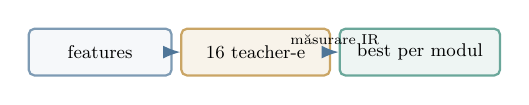
\begin{tikzpicture}[node distance=0.14cm, scale=0.74, transform shape]
\node[box, minimum width=2.45cm] (p1) {features};
\node[goldbox, right=of p1, minimum width=2.55cm] (p2) {16 teacher-e};
\node[greenbox, right=of p2, minimum width=2.75cm] (p3) {best per modul};
\draw[arrow] (p1) -- (p2);
\draw[arrow] (p2) -- node[above, font=\scriptsize]{măsurare IR} (p3);
\end{tikzpicture}
\end{center}
\end{column}
\begin{column}{0.49\textwidth}
\tiny
\begin{tabular}{@{}p{0.45\linewidth}p{0.49\linewidth}@{}}
\toprule
\textbf{Teacher} & \textbf{Semnal folosit} \\
\midrule
\texttt{never\_inline} & baseline: păstrează toate apelurile \\
\texttt{small\_callee}\\\texttt{single\_caller} & funcții mici sau folosite o singură dată \\
\texttt{constant\_argument} & constante care pot declanșa simplificări \\
\texttt{cost\_budget}\\\texttt{growth\_budget}\\\texttt{llvm\_like\_size} & bugete pentru cost și creștere de cod \\
\texttt{loop\_averse}\\\texttt{hot\_leaf}\\\texttt{aggressive\_speed} & control-flow, leaf calls, hotness proxy \\
\texttt{balanced\_score}\\\texttt{benefit\_cost\_ratio}\\\texttt{ml\_linear\_score} & scoruri beneficiu-cost pe features \\
\texttt{bandit\_ucb\_proxy}\\\texttt{rl\_value\_proxy} & proxy-uri pentru decizii secvențiale \\
\texttt{greedy\_ir\_size} & alege după IR rescris \\
\bottomrule
\end{tabular}
\end{column}
\end{columns}
\end{frame}

\begin{frame}[shrink=3]{Modele student}
\vspace{-0.05cm}
\begin{columns}[T,onlytextwidth]
\begin{column}{0.49\textwidth}
\centering
\textbf{Logistic regression}\\[-0.02cm]
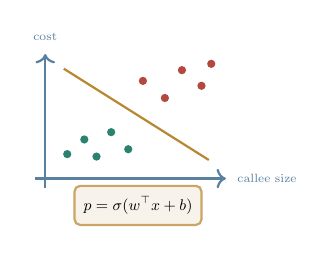
\begin{tikzpicture}[scale=0.62, transform shape]
\draw[->, thick, caiBlue!70] (-0.2,0) -- (3.7,0) node[right=3pt, font=\scriptsize]{callee size};
\draw[->, thick, caiBlue!70] (0,-0.2) -- (0,2.55) node[above=4pt, font=\scriptsize]{cost};
\foreach \x/\y in {0.45/0.5,0.8/0.8,1.05/0.45,1.35/0.95,1.7/0.6}
  \fill[caiGreen] (\x,\y) circle (2.4pt);
\foreach \x/\y in {2.0/2.0,2.45/1.65,2.8/2.22,3.2/1.9,3.4/2.35}
  \fill[caiRed] (\x,\y) circle (2.4pt);
\draw[thick, caiGold] (0.38,2.25) -- (3.35,0.38);
\node[goldbox, minimum width=2.6cm] at (1.9,-0.55) {$p=\sigma(w^\top x+b)$};
\end{tikzpicture}\\[0.16cm]
\scriptsize Un scor liniar peste vectorul de 16 features.
\end{column}
\begin{column}{0.49\textwidth}
\centering
\textbf{KNN}\\[-0.02cm]
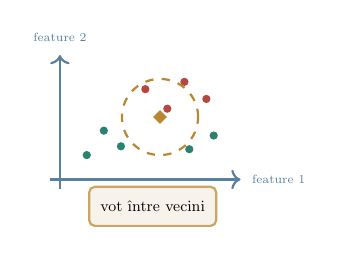
\begin{tikzpicture}[scale=0.62, transform shape]
\draw[->, thick, caiBlue!70] (-0.2,0) -- (3.7,0) node[right=3pt, font=\scriptsize]{feature 1};
\draw[->, thick, caiBlue!70] (0,-0.2) -- (0,2.55) node[above=4pt, font=\scriptsize]{feature 2};
\foreach \x/\y in {0.55/0.5,0.9/1.0,1.25/0.68,2.65/0.62,3.15/0.9}
  \fill[caiGreen] (\x,\y) circle (2.4pt);
\foreach \x/\y in {1.75/1.85,2.2/1.45,2.55/2.0,3.0/1.65}
  \fill[caiRed] (\x,\y) circle (2.4pt);
\node[diamond, draw=caiGold, fill=caiGold, inner sep=1.8pt] at (2.05,1.28) {};
\draw[dashed, thick, caiGold] (2.05,1.28) circle (0.78);
\node[goldbox, minimum width=2.6cm] at (1.9,-0.55) {vot între vecini};
\end{tikzpicture}\\[0.16cm]
\scriptsize Decizia vine din call site-uri similare.
\end{column}
\end{columns}

\vspace{0.48cm}
\begin{columns}[T,onlytextwidth]
\begin{column}{0.49\textwidth}
\centering
\textbf{Forest}\\[0.16cm]
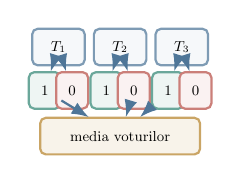
\begin{tikzpicture}[scale=0.58, transform shape]
\node[box, minimum width=1.15cm] (rA) at (0,2.2) {$T_1$};
\node[box, minimum width=1.15cm] (rB) at (1.35,2.2) {$T_2$};
\node[box, minimum width=1.15cm] (rC) at (2.7,2.2) {$T_3$};
\node[greenbox, minimum width=0.7cm] (aA) at (-0.3,1.25) {1};
\node[redbox, minimum width=0.7cm] (bA) at (0.3,1.25) {0};
\node[greenbox, minimum width=0.7cm] (aB) at (1.05,1.25) {1};
\node[redbox, minimum width=0.7cm] (bB) at (1.65,1.25) {0};
\node[greenbox, minimum width=0.7cm] (aC) at (2.4,1.25) {1};
\node[redbox, minimum width=0.7cm] (bC) at (3.0,1.25) {0};
\draw[arrow] (rA) -- (aA);
\draw[arrow] (rA) -- (bA);
\draw[arrow] (rB) -- (aB);
\draw[arrow] (rB) -- (bB);
\draw[arrow] (rC) -- (aC);
\draw[arrow] (rC) -- (bC);
\node[goldbox, minimum width=3.5cm] (vote) at (1.35,0.25) {media voturilor};
\draw[arrow] (aA) -- (vote);
\draw[arrow] (bB) -- (vote);
\draw[arrow] (aC) -- (vote);
\end{tikzpicture}\\[0.16cm]
\scriptsize Media voturilor stabilizează decizia.
\end{column}
\begin{column}{0.49\textwidth}
\centering
\textbf{MLP}\\[0.16cm]
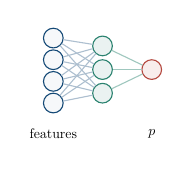
\begin{tikzpicture}[scale=0.50, transform shape]
\foreach \y/\n in {0/iA,0.55/iB,1.1/iC,1.65/iD}
  \node[circle, draw=caiBlue, fill=softGray, minimum size=5mm] (\n) at (0,\y) {};
\foreach \y/\n in {0.25/hA,0.85/hB,1.45/hC}
  \node[circle, draw=caiGreen, fill=caiGreen!10, minimum size=5mm] (\n) at (1.25,\y) {};
\node[circle, draw=caiRed, fill=caiRed!10, minimum size=5mm] (o) at (2.5,0.85) {};
\foreach \i in {iA,iB,iC,iD} \foreach \h in {hA,hB,hC} \draw[caiBlue!35] (\i) -- (\h);
\foreach \h in {hA,hB,hC} \draw[caiGreen!45] (\h) -- (o);
\node[align=center, font=\normalsize, fill=white, inner sep=1.4pt] at (0,-0.78) {features};
\node[align=center, font=\normalsize, fill=white, inner sep=1.4pt] at (2.5,-0.78) {$p$};
\end{tikzpicture}\\[0.16cm]
\scriptsize Straturile ascunse modelează interacțiuni între features.
\end{column}
\end{columns}
\end{frame}

\begin{frame}[shrink=3]{Cum se face rescrierea IR}
\begin{columns}[T,onlytextwidth]
\begin{column}{0.46\textwidth}
\begin{enumerate}
  \item Citesc LLVM IR textual.
  \item Elimin \texttt{noinline}: funcția poate fi inlined.
  \item Clonez callee-ul selectat cu nume unic.
  \item Marchez clona cu \texttt{alwaysinline}.
  \item Redirecționez numai apelul selectat.
  \item Rulez LLVM \texttt{opt}: aplică pass-urile de optimizare pe IR.
\end{enumerate}
\end{column}
\begin{column}{0.50\textwidth}
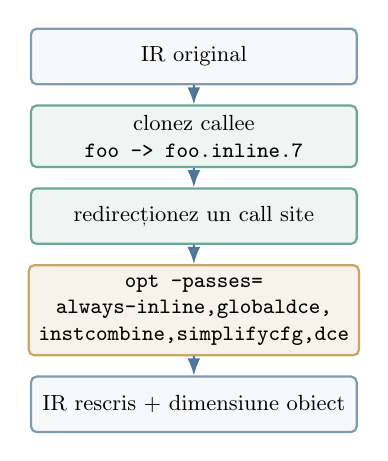
\begin{tikzpicture}[node distance=0.28cm, scale=0.88, transform shape]
\node[box, minimum width=4.7cm] (a) {IR original};
\node[greenbox, below=of a, minimum width=4.7cm] (b) {clonez callee\\\texttt{foo -> foo.inline.7}};
\node[greenbox, below=of b, minimum width=4.7cm] (c) {redirecționez un call site};
\node[goldbox, below=of c, minimum width=4.7cm] (d) {\texttt{opt -passes=}\\\texttt{always-inline,globaldce,}\\\texttt{instcombine,simplifycfg,dce}};
\node[box, below=of d, minimum width=4.7cm] (e) {IR rescris + dimensiune obiect};
\draw[arrow] (a) -- (b);
\draw[arrow] (b) -- (c);
\draw[arrow] (c) -- (d);
\draw[arrow] (d) -- (e);
\end{tikzpicture}
\end{column}
\end{columns}
\vspace{0.2cm}
\scriptsize
\texttt{always-inline}: materializează apelurile marcate; \texttt{globaldce}: elimină funcții/globale nefolosite; \texttt{instcombine}: simplifică instrucțiuni; \texttt{simplifycfg}: curăță control-flow-ul; \texttt{dce}: elimină cod mort.
\end{frame}

\begin{frame}{Exemplu vizual: ce se schimbă în graful de apeluri}
\centering
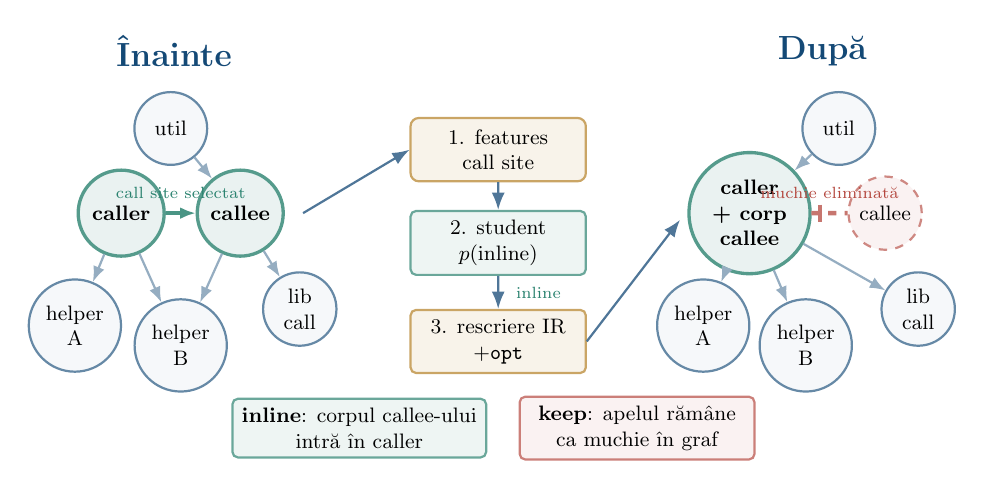
\begin{tikzpicture}[
  scale=0.84, transform shape,
  callnode/.style={circle, draw=caiBlue!65, fill=softGray, thick, minimum size=11mm, align=center, font=\small},
  focusnode/.style={circle, draw=caiGreen!80, fill=caiGreen!10, very thick, minimum size=13mm, align=center, font=\small\bfseries},
  gone/.style={circle, draw=caiRed!65, fill=caiRed!7, thick, dashed, minimum size=11mm, align=center, font=\small},
  pipe/.style={rounded corners=3pt, draw=caiGold!75, fill=caiGold!10, thick, align=center, inner sep=5pt, font=\small},
  edgekeep/.style={-{Latex[length=2mm]}, draw=caiBlue!45, thick},
  edgeinline/.style={-{Latex[length=2mm]}, draw=caiGreen!85, ultra thick},
  edgeremoved/.style={draw=caiRed!75, ultra thick, dashed}
]

\node[font=\Large\bfseries, text=caiBlue] at (-4.9,3.45) {Înainte};
\node[font=\Large\bfseries, text=caiBlue] at (4.9,3.45) {După};

% Before graph
\node[focusnode] (caller) at (-5.7,1.0) {caller};
\node[focusnode] (callee) at (-3.9,1.0) {callee};
\node[callnode] (h1) at (-6.4,-0.7) {helper\\A};
\node[callnode] (h2) at (-4.8,-1.0) {helper\\B};
\node[callnode] (h3) at (-3.0,-0.45) {lib\\call};
\node[callnode] (h4) at (-4.95,2.28) {util};
\draw[edgeinline] (caller) -- node[above=2pt, font=\scriptsize, text=caiGreen] {call site selectat} (callee);
\draw[edgekeep] (caller) -- (h1);
\draw[edgekeep] (caller) -- (h2);
\draw[edgekeep] (callee) -- (h2);
\draw[edgekeep] (callee) -- (h3);
\draw[edgekeep] (h4) -- (callee);

% Decision pipeline
\node[pipe, minimum width=2.65cm] (feat) at (0,1.96) {1. features\\call site};
\node[greenbox, minimum width=2.65cm] (model) at (0,0.55) {2. student\\$p(\mathrm{inline})$};
\node[goldbox, minimum width=2.65cm] (rewrite) at (0,-0.94) {3. rescriere IR\\+\texttt{opt}};
\draw[arrow] (feat) -- (model);
\draw[arrow] (model) -- node[right=4pt, font=\scriptsize, text=caiGreen]{inline} (rewrite);
\draw[arrow] (-2.95,1.0) -- (feat.west);
\draw[arrow] (rewrite.east) -- (2.75,0.9);

% After graph
\node[focusnode, minimum size=15mm] (caller2) at (3.8,1.0) {caller\\+ corp\\callee};
\node[gone] (callee2) at (5.85,1.0) {callee};
\node[callnode] (a1) at (3.1,-0.7) {helper\\A};
\node[callnode] (a2) at (4.65,-1.0) {helper\\B};
\node[callnode] (a3) at (6.35,-0.45) {lib\\call};
\node[callnode] (a4) at (5.15,2.28) {util};
\draw[edgeremoved] (caller2) -- node[above=2pt, font=\scriptsize, text=caiRed] {muchie eliminată} (callee2);
\draw[caiRed!75, ultra thick] ($(caller2)!0.52!(callee2)+(0,0.13)$) -- ($(caller2)!0.52!(callee2)+(0,-0.13)$);
\draw[edgekeep] (caller2) -- (a1);
\draw[edgekeep] (caller2) -- (a2);
\draw[edgekeep] (caller2) -- (a3);
\draw[edgekeep] (a4) -- (caller2);

\node[greenbox, minimum width=3.55cm] at (-2.1,-2.25) {\textbf{inline}: corpul callee-ului\\intră în caller};
\node[redbox, minimum width=3.55cm] at (2.1,-2.25) {\textbf{keep}: apelul rămâne\\ca muchie în graf};
\end{tikzpicture}
\end{frame}

\begin{frame}[shrink=4]{Rezultate}
\vspace{-0.15cm}
\begin{columns}[T,onlytextwidth]
\begin{column}{0.50\textwidth}
\centering
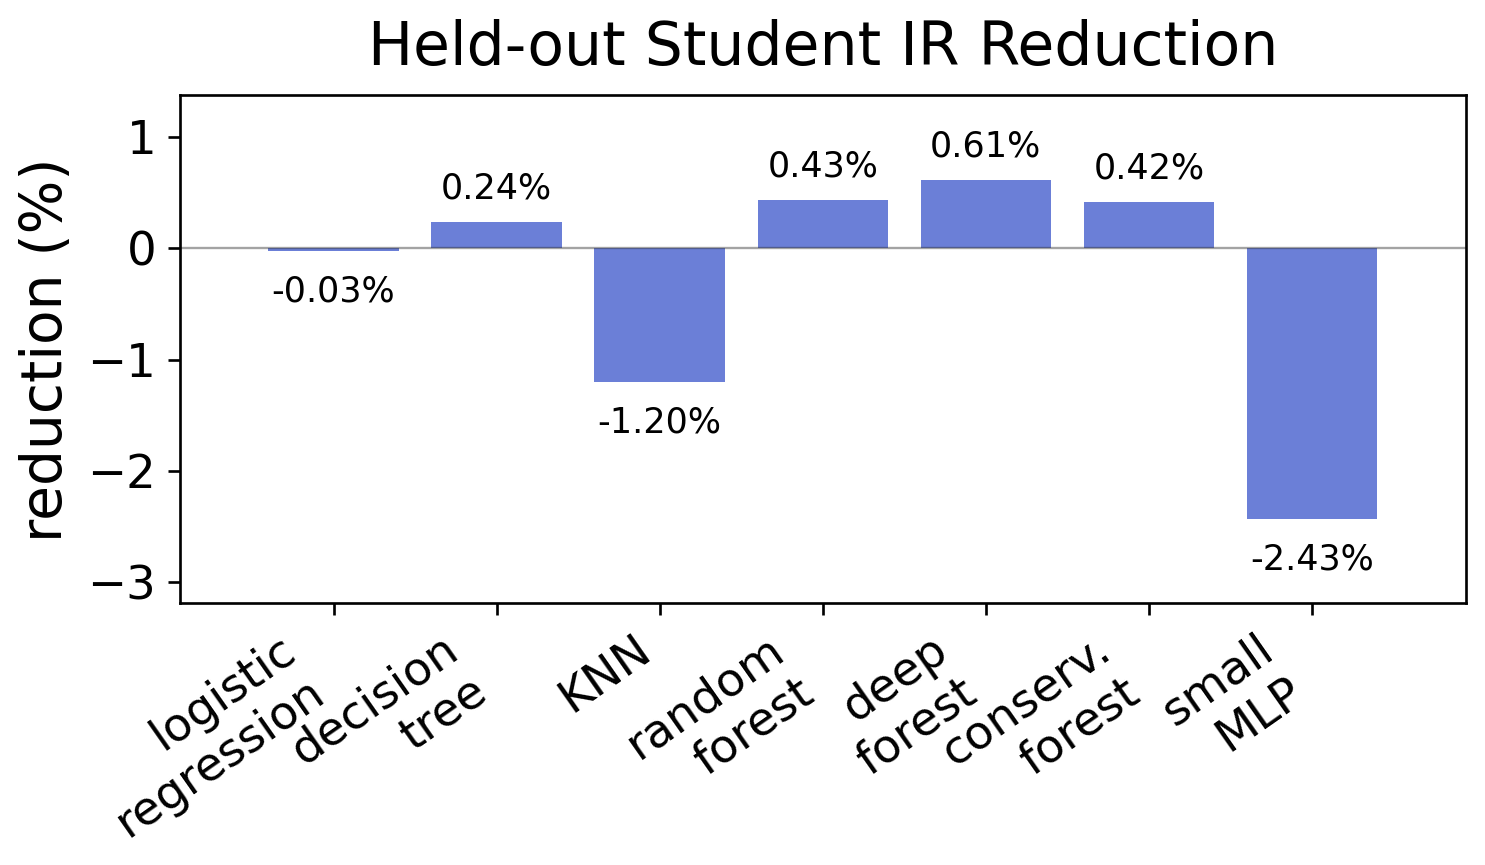
\includegraphics[width=\linewidth,height=0.36\textheight,keepaspectratio]{student_ir_reduction.png}
\end{column}
\begin{column}{0.50\textwidth}
\centering
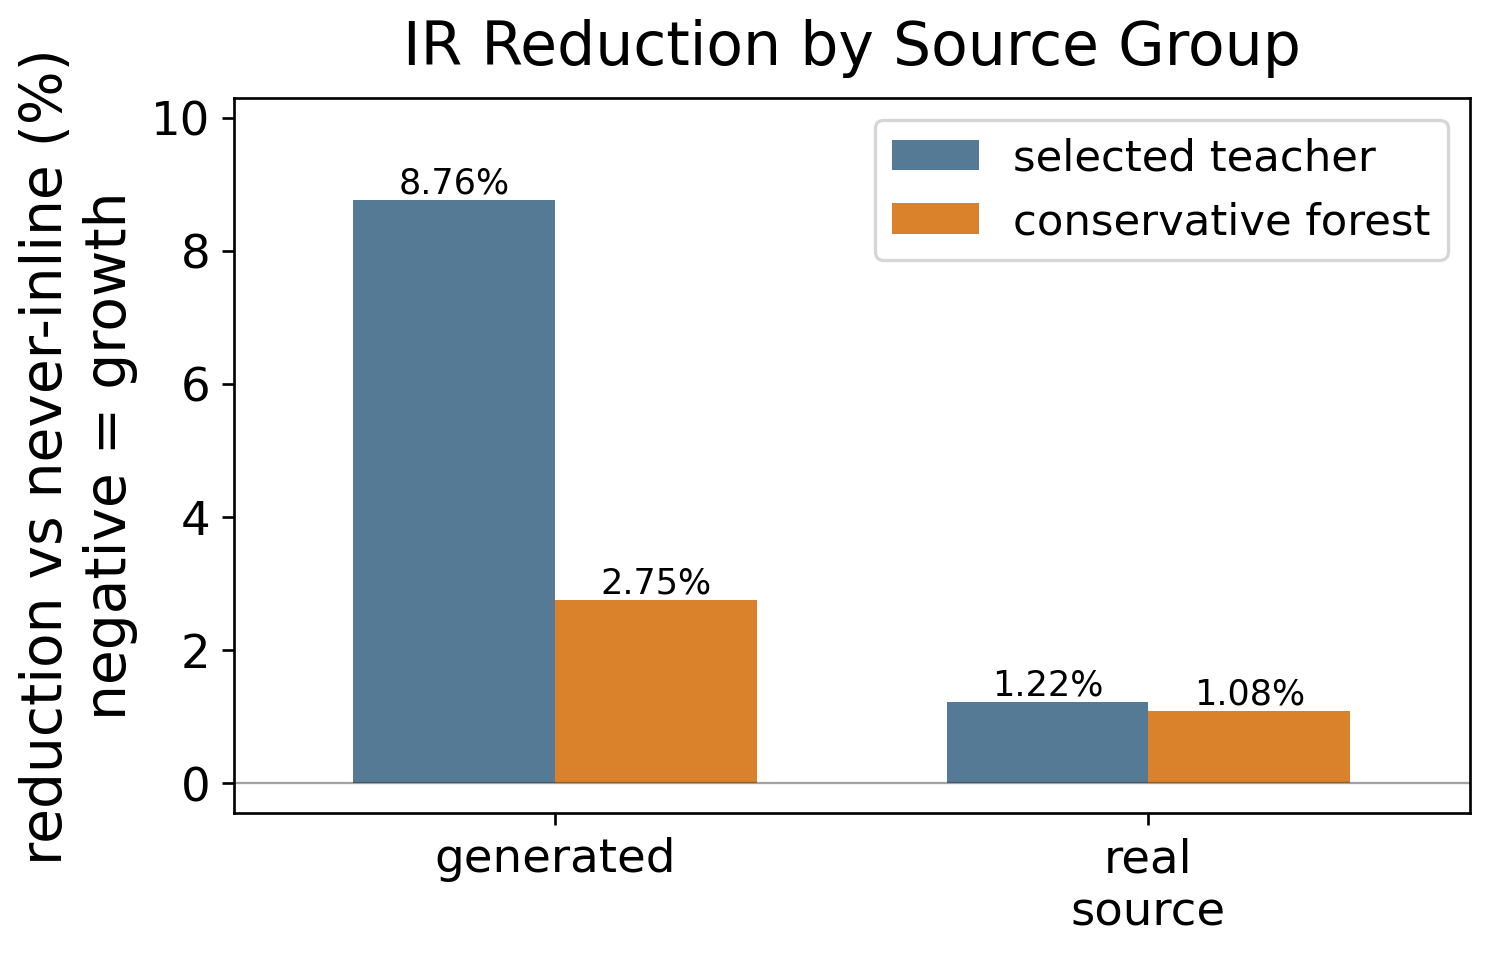
\includegraphics[width=\linewidth,height=0.36\textheight,keepaspectratio]{source_group_ir_reduction.png}
\end{column}
\end{columns}
\vspace{0.08cm}
\begin{columns}[T,onlytextwidth]
\begin{column}{0.49\textwidth}
\begin{itemize}
  \item 10.394 call site-uri analizate.
  \item Held-out: cel mai bun model obține \textbf{0,61\%} reducere IR.
  \item Rulare principală: \textbf{conservative forest} are \textbf{1,18\%} reducere totală IR.
\end{itemize}
\end{column}
\begin{column}{0.49\textwidth}
\begin{itemize}
  \item Selected-teacher pe held-out: \textbf{1,10\%} reducere IR.
  \item Surse reale: \textbf{deep forest} obține \textbf{1,08\%} reducere totală IR.
  \item Evaluarea pune accent pe rescrierea IR și folosește match-ul de etichete ca diagnostic.
\end{itemize}
\end{column}
\end{columns}
\end{frame}

\begin{frame}{Demo}
\begin{columns}[T,onlytextwidth]
\begin{column}{0.47\textwidth}
\textbf{Comandă}
\begin{block}{}
\small\texttt{python3 scripts/run.py demo}
\end{block}
\textbf{Ce arată}
\begin{itemize}
  \item compilează module C++ generate în LLVM IR;
  \item extrage features pentru call site-uri;
  \item aplică decizii prin același mecanism clone-and-\texttt{opt};
  \item scrie decizii (\texttt{0=keep}, \texttt{1=inline}) și IR rescris în \texttt{out/demo/}.
\end{itemize}
\end{column}
\begin{column}{0.49\textwidth}
\centering
\href{run:complete_optimizing_inlining_dem.mp4}{%
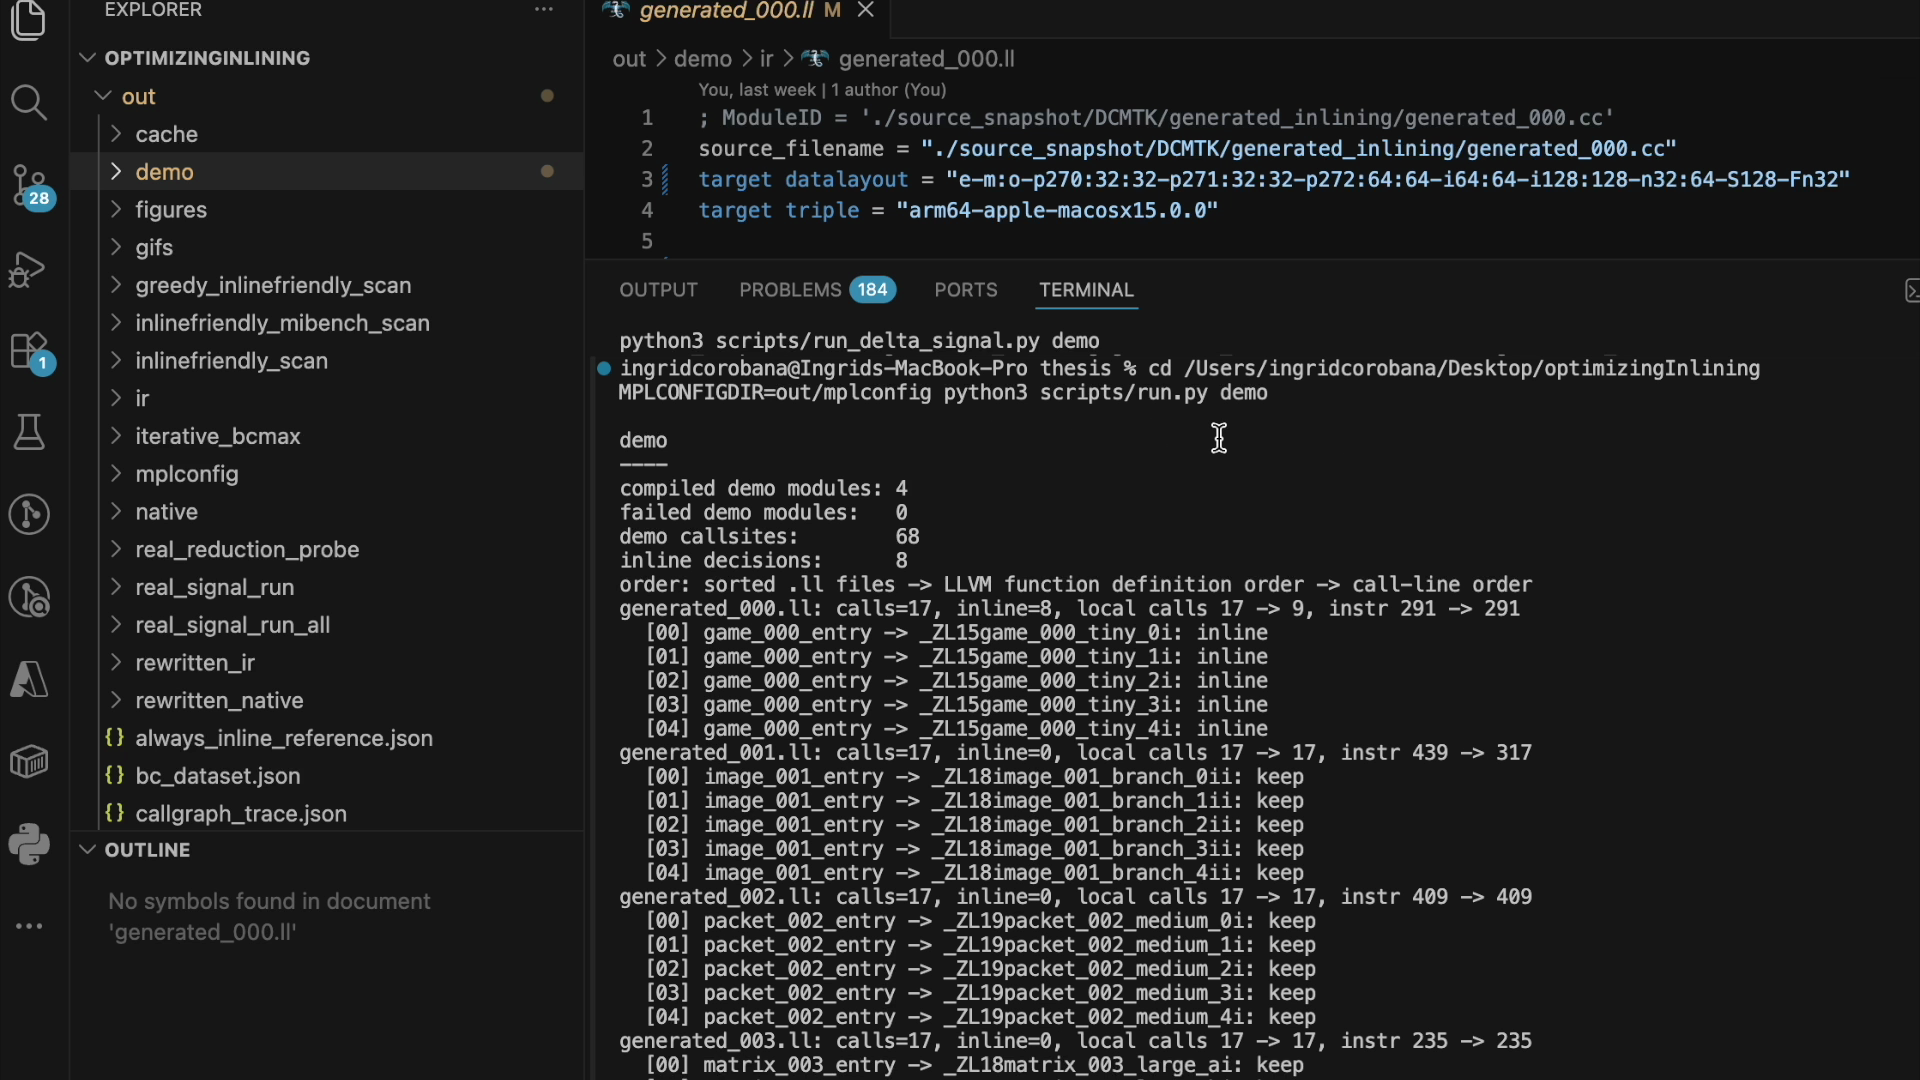
\includegraphics[width=\linewidth,height=0.58\textheight,keepaspectratio]{complete_optimizing_inlining_demo_frame.png}}
\vspace{0.05cm}
\scriptsize Demo: \texttt{complete\_optimizing\_inlining\_dem.mp4}
\end{column}
\end{columns}
\end{frame}

\begin{frame}[shrink=4]{Limitări și concluzii}
\begin{columns}[T,onlytextwidth]
\begin{column}{0.49\textwidth}
\textbf{Limitări}
\begin{itemize}
  \item prototip peste LLVM IR, cu integrare LLVM pass ca pas următor;
  \item rescriere textuală de IR, cu aceeași selecție deterministă a call site-urilor;
  \item metrici pe instrucțiuni IR și obiect \texttt{.text};
  \item problemă secvențială aproximată offline: deciziile sunt alese pe seturi fixe de call site-uri.
\end{itemize}
\end{column}
\begin{column}{0.49\textwidth}
\textbf{Concluzii}
\begin{itemize}
  \item Am demonstrat un workflow reproductibil pentru inlining ghidat de ML.
  \item Contribuția teoretică: formularea inlining-ului ca problemă offline de imitare, cu profesori euristici și selecție per modul.
  \item Contribuția practică: legătura dintre decizii ML și artefacte de compilator inspectabile.
  \item Pași următori: benchmark-uri mai mari, profesori mai puternici, integrare ca LLVM pass.
\end{itemize}
\end{column}
\end{columns}
\end{frame}

\end{document}
